\documentclass{article}

\usepackage { fancyhdr } % headers and footers
\usepackage[headsep = 2.75cm, headheight = 0cm] { geometry } % showframe, margins
\usepackage { graphicx } % images
\usepackage[export] { adjustbox } % right or left for images
\usepackage[hidelinks] { hyperref } % hyperlinks
\usepackage { sectsty } % section font
\usepackage { array } % C macro
\usepackage { tikz }
\usepackage { multicol }

\geometry {
    a4paper,
    total={180mm,220mm},
    left=20mm,
    top=30mm,
    bottom=30mm
}

\pagestyle{fancy}
\fancyhf{}
\renewcommand{\headrulewidth}{0pt} % no bottom border for header

% macro to center and wrap text in table cell
\newcolumntype{C}[1]{>{\centering\let\newline\\\arraybackslash\hspace{0pt}}m{#1}}
\newcolumntype{L}[1]{>{\raggedright\let\newline\\\arraybackslash\hspace{0pt}}m{#1}}

% font size of a section
\sectionfont{\fontsize{15}{15}\selectfont\centering}

% header
\lhead { \small Bucharest,  \\ Romania  }
\chead { \textbf{ \Large Mihai-Bogdan Vîlculescu } }
\rhead { 
    \href{https://www.github.com/BogdanVM} {\includegraphics[width = .80cm, height = .80cm, right]{git2.png} }    
    \small bogdan.vilculescu@gmail.com \\
    \small (+40)724073974 }

\lfoot { \href{https://www.linkedin.com/in/bogdan-vilculescu/} { \includegraphics[width = .80cm, height = .80cm, left]{linkedin.png} } }

% main document
\begin{document}
    
    \begin{multicols}{2}
    
    % Experience Section
    \section*{ Experience }
    \large \textit{- Jun 2021 - Present} - \textbf{\textit{Frontend Developer}} at \textbf{Beecoded}
        \vspace{0.35cm}\\ \normalsize \indent During this time, I specialised in frontend development (\textbf{Angular, React, Ionic Framework})
        \\ \indent This experience has also helped me develop my soft skills, as I was required from time to time to \textbf{interact with clients} and to \textbf{manage tight deadlines}.
        \\ \indent I feel like the most improved skills from this period were:
        \begin{itemize}
            \item Frontend JavaScript frameworks (Angular, React)
            \item Time management
            \item Communication skills
            \item Project management
        \end{itemize}
        
    \vspace{0.5cm}
    \large \textit{- Aug 2020 - Jun 2021} - \textbf{\textit{Full Stack Developer}} at \textbf{Codesilk}
        \vspace{0.35cm}\\ \normalsize \indent I worked on different web and mobile projects. During this time, I've worked with both backend and frontend technologies:
        \begin{itemize}
            \item Laravel / Node.js / Wordpress;
            \item Angular / React
        \end{itemize}
    
    % Volunteering Section
    \section*{ Volunteering }
        
        \large \textit{- Mar 2018 - Jan 2020} - \textbf{\textit{Volunteer}} at \textbf{Codette}
        \\ \\ \normalsize \indent As I empathize with the organisation's purpose (the empowerment of women to pursue careers in technology), I joined in as a volunteer in March 2018. My involvement consisted of providing assistance with organizing different events, supported by Codette, such as the Code For All Summit in 2018.
        
        \vspace{0.5cm}
        \large \textit{- Nov 2018 - January 2019} - \textbf{\textit{Tutor of C}} at \textbf{University of Bucharest}
        \vspace{0.35cm}\\  \normalsize \indent Tutoring consists of assisting first year students with a certain subject. In 2018, I participated as a tutor of C language, helping younger students understand this subject.
        
        \vspace{0.5cm}
        \large \textit{- Feb 2019 - June 2019} - \textbf{\textit{Tutor of OOP}} at \textbf{University of Bucharest}
        \vspace{0.35cm}\\  \normalsize \indent During the second semester, in 2019, I became tutor of OOP where I helped students with grasping the basic concepts of OOP (Encapsulation, Inheritance, Polymorphism), illustrated in C++.
        

    % Education Section
    \section*{Education}
        \large \textit{- Oct 2017 - Jun 2020} - \textbf{\textit{BS Degree}} \\ \textbf{Faculty of Math and Comp Science, University of Bucharest}
        \vspace{0.35cm}\\ \normalsize\indent Studied   Algorithms,   Programming   Languages   (C,   C++,Java), Operating Systems, Web Technologies (Frontend).
        

    % Personal Projects
    \section*{Personal Projects}
        \textbf{\textit{- La Vot:}} \textbf{Technologies used:} HTML, CSS, PHP and JavaScript.
        \vspace{0.35cm}\\ \textbf{\textit{- BrioBAC:}} \textbf{Technologies used (Android):} Java, XML,SQL, Php.

    % Additional Experience Section
    \section*{Additional Experience}
        \textbf{\textit{- Google Digital Workshop - Java Training (November 2018 - February 2019)}}
        \vspace{0.35cm}\\ \textbf{\textit{- Google Digital Workshop - Android Advanced Training (March 2019 - June 2019)}};
        \vspace{0.35cm}\\ \textbf{\textit{- Pedagogical Module(October 2018 - Jun 2020):}} Attended the pedagogical module held at our univeristy for people who wanted to become teachers. I do not necessarily intend to pursue a career in teaching, but I believe this is a great opportunity to learn and explore new things. 
    
    % Languages and Technologies Section
    \section*{Languages and Technologies}
        \begin{multicols}{2}
        \begin{itemize}
            \item[] \scriptsize 
                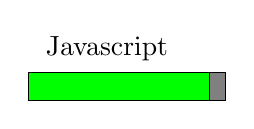
\begin{tikzpicture}
                    \node [anchor=west] at (.1,.65) {Javascript};
                    \draw [fill=gray] (0,0) rectangle (2.5,.35);
                    \draw [fill={rgb:red,0;green,1;blue,0}] (0,0) rectangle (2.3, .35);
                \end{tikzpicture}
                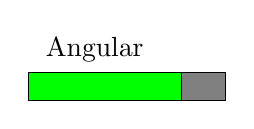
\begin{tikzpicture}
                    \node [anchor=west] at (.1,.65) {Angular};
                    \draw [fill=gray] (0,0) rectangle (2.5,.35);
                    \draw [fill={rgb:red,0;green,1;blue,0}] (0,0) rectangle (1.95,.35);
                \end{tikzpicture}
                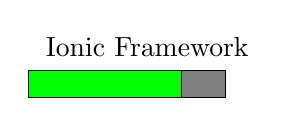
\begin{tikzpicture}
                    \node [anchor=west] at (.1,.65) {Ionic Framework};
                    \draw [fill=gray] (0,0) rectangle (2.5,.35);
                    \draw [fill={rgb:red,0;green,1;blue,0}] (0,0) rectangle (1.95,.35);
                \end{tikzpicture}
                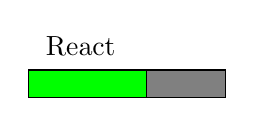
\begin{tikzpicture}
                    \node [anchor=west] at (.1,.65) {React};
                    \draw [fill=gray] (0,0) rectangle (2.5,.35);
                    \draw [fill={rgb:red,0;green,1;blue,0}] (0,0) rectangle (1.5,.35);
                \end{tikzpicture}
                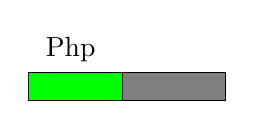
\begin{tikzpicture}
                    \node [anchor=west] at (.1,.65) {Php};
                    \draw [fill=gray] (0,0) rectangle (2.5,.35);
                    \draw [fill={rgb:red,0;green,1;blue,0}] (0,0) rectangle (1.2,.35);
                \end{tikzpicture}
            
            \item[]
                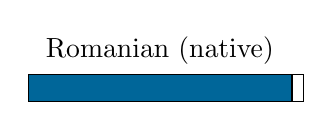
\begin{tikzpicture}
                    \node [anchor=west] at (.1,.65) {Romanian (native)};
                    \draw [fill=white] (0,0) rectangle (3.5,.35);
                    \draw [fill={rgb:red,0;green,2;blue,3}] (0,0) rectangle (3.35,.35);
                \end{tikzpicture}
                
\begin{tikzpicture}
                    \node [anchor=west] at (.1,.65) {English (CAE certificate)};
                    \draw [fill=white] (0,0) rectangle (3.5,.35);
                    \draw [fill={rgb:red,0;green,2;blue,3}] (0,0) rectangle (2.85,.35);
                \end{tikzpicture}
                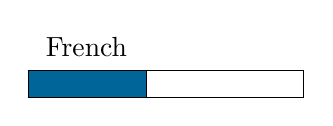
\begin{tikzpicture}
                    \node [anchor=west] at (.1,.65) {French};
                    \draw [fill=white] (0,0) rectangle (3.5,.35);
                    \draw [fill={rgb:red,0;green,2;blue,3}] (0,0) rectangle (1.5,.35);
                \end{tikzpicture}
            
        \end{itemize}
        \end{multicols}
    
    % Hobbies and Interests Section
    \section*{Hobbies and Interests}
        \begin{multicols}{2}
        \begin{itemize}
            \item Listening to music;
            \item Science Fiction;
            \item Strategy Games;
            \item Politics.
        \end{itemize}
        \end{multicols}
        \end{multicols}
\end{document}
